% UTF-8 encoding
\documentclass[9pt, dvipsnames]{beamer} %
\usetheme[secheader]{Boadilla} 
\usecolortheme{beaver} 
\usefonttheme{professionalfonts} 
\usepackage{times}
\usepackage{amsmath,amsfonts,amssymb,amsthm}
\usepackage{geometry}
\usepackage{verbatim}
\usepackage{anyfontsize}
\usepackage{subcaption} % 子图片
\usepackage{graphicx} % 图片
\usepackage[export]{adjustbox}
\setbeamertemplate{caption}[numbered]
\newcounter{saveenumi}
\resetcounteronoverlays{saveenumi}
\usepackage[multidot]{grffile} % 允许文件名带多个点
\usepackage{tabularx} % 表格
\usepackage{tikz}
\vfuzz=30pt

\title{Robust Topological Inference}
\author[048985]{Tom Norman}
\date{July 1, 2020}
\def\norm#1{\mathopen\| #1 \mathclose\|}% use instead of $\|x\|$
\newcommand {\image}[3] {
    \begin{figure}
        \begin{center}
		\includegraphics[width=\textwidth,height=#3\textheight,keepaspectratio]{imgs/#1}
		\caption{#2}
        \end{center}
    \end{figure}
}

\DeclareMathOperator*{\argmax}{arg\,max}

\begin{document}

    \everymath{\displaystyle}

    \begin{frame}
        \titlepage
    \end{frame}

    \begin{frame}
        \frametitle{\textbf{Overview}}
        \tableofcontents
    \end{frame}


    \section{Distance Function Offset}\label{sec:dfo}
    \begin{frame}
        \frametitle{\textbf{Distance Function Offset}}
	\centerline{Using a distance function to discover the persistent homology of the data}
	\image{only_distance.png}{2 circles and L2 distance of every point in $\mathbb{R}^2$ to the nearest sample}{0.9}
    \end{frame}
    \begin{frame}
	\begin{itemize}
		\item
			Given data $X = \{ x_1, x_2, ..., x_n \} \in \mathbb{R}^d$
		\item
			$\forall x \in \mathbb{R}^d \text{ compute } d_X(x) = \min_{x_i \in X} \norm{x_i - x}_2$
		\item
			Run persistent homology for fucntions to get filtarations of sublevel sets $L_t = \{ x : d_X(x) \leq t \}$
	\end{itemize}
	\image{sublevel_demo.jpg}{A circle, its L2 distance function and the sublevel set for t=0.25}{0.6}
	\end{frame}

	\section{Persistence Diagram}\label{sec:pd}
	\begin{frame}
		\frametitle{\textbf{Persistence Diagram}}
		\centerline{A way to visualize persistent homology}
		\image{sphere_ph.png}{Persistence diagram of the unit sphere}{0.9}
	\end{frame}
	\begin{frame}
		\begin{itemize}
			\item
				For $t: 0 \to \infty$ find birth and death (denoted $b_i$ and $d_i$) of each homology feature (connected component, hole, void, etc.)
			\item
				Create 2D graph from those $b_i, d_i$
			\item
				Note that $b_i \leq$ $d_i$
		\end{itemize}

		\image{distFct_ph_demo.png}{Persistence diagram of 2 circles}{0.6}
	\end{frame}


	\section{Outliers (Motivation)}\label{sec:out}
	\begin{frame}
		\frametitle{\textbf{Outliers (Motivation)}}
		\centering
			L2 distance is very sensitive to outliers\\
	    \begin{figure}
		    \centering
			 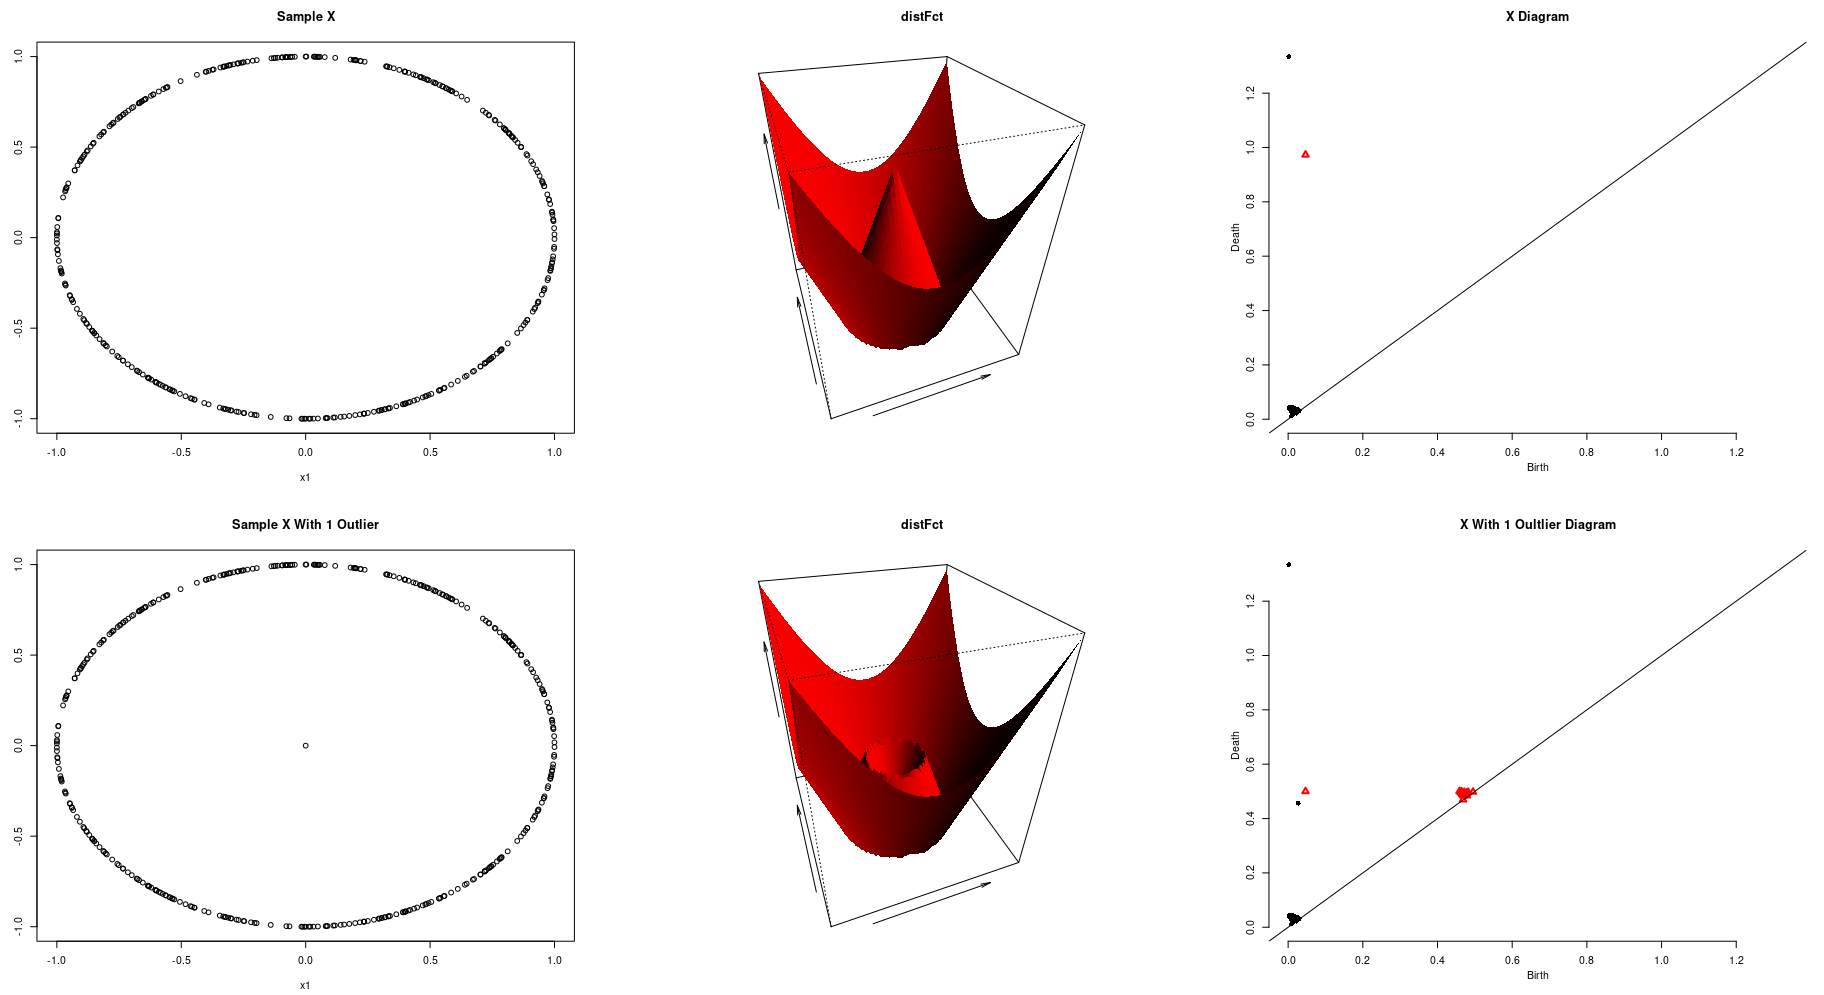
\includegraphics[width=\linewidth]{imgs/outlier_demo.png}
		    \caption{400 samples of the unit circle, the lower plot with 1 extra outlier}
	    \end{figure}
	\end{frame}

	\section{Distance to (Probability) Measure}\label{sec:dtm}
	\begin{frame}
		\frametitle{\textbf{Distance to (Probability) Measure}}
		\centerline{Smooth function which is robust to outliers and noise}
		\image{mechanical_outliers.png}{Left: Point cloud of a mechanical part with noise, Right: Reconstruction using DTM}{0.9}
	\end{frame}
	\begin{frame}
		\begin{itemize}
			\item
				Define $G_x(t) = \mathbb{P} \left( \norm{X - x} \leq t \right)$- probability of a ball with radius $t$ around point $x$

			\item
				Given $m_0 \in (0,1)$ (smoothing parameter) \\
				\centerline{$DTM_X^{m_0}(x) = \sqrt{\frac{1}{m_0} \int_0^{m_0} \left( G_x^{-1} (u) \right)^2 du}$} \item
				We'll assign each data point $\frac{1}{n}$ probability mass 
				and take $m_0 = \frac{k}{n}$\\
				\centerline{$DTM_X^{m_0}(x) = d_X^k(x) = \sqrt{\frac{1}{k} \sum_{x_i \in kNN_X(x)} \norm{x_i -x}^2}$}
		\end{itemize}
	\end{frame}
	\begin{frame}
		\image{dtm_demo.png}{400 samples, k=2}{0.9}
	\end{frame}

    \section{Bottleneck Distance}\label{sec:bnd}
    \begin{frame}
	    \centerline{Distance between 2 persistence diagrams}
        \frametitle{\textbf{Bottleneck Distance}}
	\image{bottleneck_distance_example.png}{The bottleneck distance is the longest red edge}{0.7}
    \end{frame}
    \begin{frame}
	\begin{itemize}
		\item
			Given 2 persistent diagrams $D_1, D_2$ (including the diagonal, where birth==death)\\
			denote bottleneck distance as\\
		\centerline{$W_\infty (D_1, D_2) = \min_{g: D_1 \to D2} \sup_{z \in D_1} \norm{z - g(z)}_\infty$}
		(g is a bijection)
		\item
			In words: the maximum distance between the features of the 2 diagrams,\\
			after minimizing over all possible pairings of the features (including the diagonal)
	\end{itemize}
    \end{frame}

    \section{Significance of Features Using Bootstrapping}\label{sec:boot}
    \def\dk{d_X^k}
    \begin{frame}
	    \frametitle{\textbf{Significance of Features Using Bootstrapping}}
	    \center
		Quantify the confidence that the homology feature came from the underlying shape
		\image{bootstrapping.png}{2 overlapping unit circles. Only 3 holes are statistically significant.}{0.9}
    \end{frame}
    \begin{frame}
	    \begin{itemize}
		    \item
			    Given $X$ and $k$ compute $\dk$
		    \item
			    Sample n points at random from X with replacement (denoted $X_i^*$),\\
			    and compute $\theta_i^* =  \sqrt{n} \norm{\dk(x) - d_{X_i^*}^k(x)}_\infty \propto W_\infty \left( D_X, D_{X_i^*} \right)$
		    \item
			    Repeat last step B times
		    \item
			    Given $\alpha$ compute $t_\alpha = \min_t \left\{ \sum_{i=1}^B \text{\LARGE{1}}\{\theta_i^* \geq t\} \leq \alpha B \right\}$:\\
			    minimum t for which there are at most $\alpha B$ bigger $\theta_i^*$'s.
		    \item
			    $\forall$ feature $i$:\\
			    \centerline{if $|b_i-d_i| > \frac{2t_\alpha}{\sqrt{n}}$, then the feature is $\alpha$-significant}
	    \end{itemize}

    \end{frame}
%    \begin{frame}
%	    \image{bph.png}{$t_\alpha$ = 0.5}{1}
%    \end{frame}

    \section{Choosing Smoothing Parameter}\label{sec:param}
    \begin{frame}
	    \frametitle{\textbf{Choosing Smoothing Parameter}}
	    \centerline{Choose $m_0$ that maximizes the total amount of significant information}
	    \image{maxpersistence_example.png}{400 samples from unit circle + 100 samples from normal distribution, $k$ = [1:10:191]}{0.9}
    \end{frame}
    \begin{frame}
	    \begin{itemize}
		    \item
			    Let $\ell_i(m_0)$ be the lifetime of feature $i$ with smoothing parameter $m_0$
		    \item
			    Given $\frac{t_\alpha}{\sqrt{n}}$, define:\\
			    \centerline{$ N(m_0) = \# \left\{ i: \ell_i(m_0) > \frac{2t_\alpha}{\sqrt{n}} \right\}$}
			    \centerline{(Number of $\alpha$-significant features for given $m_0$)}
			    and:\\
			    \centerline{$ S(m_0) = \sum_i \left[ \ell_i(m_0) - \frac{2t_\alpha}{\sqrt{n}} \right]_+ $}
			    \centerline{(Sum of distances from $\alpha$-significance for given $m_0$)}
		    \item
			    $ m_{opt} = \argmax_{m_0} N(m_0) \text{\textbf{ or }} \argmax_{m_0} S(m_0) $
	    \end{itemize}
    \end{frame}

	\section{Further Work}\label{sec:work}
	\begin{frame}
	    \frametitle{\textbf{Further Work}}
		Would like to test DTM vs. L2 distance on real world data:
		\begin{itemize}
			\item
				Point cloud MNIST
			\item
				Find safe neighborhoods in Vancouver and Boston
			\item
				Movies - what is uncommon length, rating, etc for each genere
			\item
				Ideas?
		\end{itemize}
		\image{mnist.png}{Point cloud MNIST}{0.5}
	\end{frame}

\end{document}
